
In the next part we vary given parameters in order to make a sensitivity analysis. This takes a lot of simulation runs, and we demonstrate the of use parallel computing to speed up execution.

In this exemplary sensitivity study we will vary the insertion angle of the tap and basal root, and look at the resulting change in mean root tip depth and root tip radial distance. 

\lstinputlisting[language=Python, caption=Example 2f]{examples/example2f_sensitivity.py}

\begin{itemize}

\item[12-20] Defines a function to set all standard deviations proportional to the parameter values. We use this function in the following to set the standard deviation to zero everywhere. 

\item[23-29] Parameters of the analysis. $N$ denotes the resolution of the parameter we vary, and $runs$ the number of iterations, i.e. a total of $N\cdot runs$ simulations are performed. In L29 we define the insertion angle to be varied linearly between 0 and $\pi/2$.

\item[33-52] Definition of a function that performs the simulation and returns mean root tip depth and radial distance. First we create a root system and set the standard deviation to zero L34-L36. L37, amd L39 sets the insertion angle. L41 initializes the root system and states that basal root are of root type 1 (same as tap root). The False value turns of verbosity to avoid any outputs to the console. L42 performs the simulation. L44-L51 calculates the mean root tip depth and radial distance. 

\item[55-73] This section performs the computation of all simulation runs. L55-56 preallocates the resulting arrays. L62-L68 performs the parallel computations, index $i$ is the index of the insertion angle. L71-73 calculates the mean values per simulation run.

\item[74-83] Creates the resulting Figure \ref{fig:sensitivity}. Note that the resulting curves become smoother, if the number of runs is increased (L28).

\end{itemize}

% 
% \begin{figure}
% \centering
% 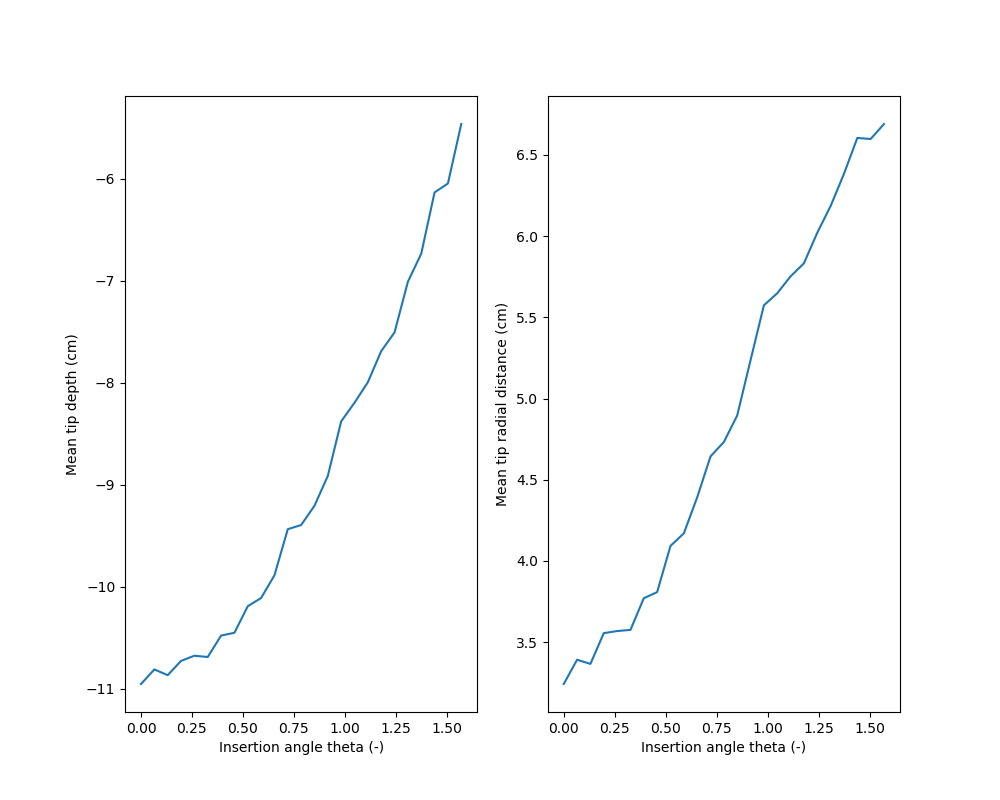
\includegraphics[width=0.7\textwidth]{example_4b.png}
% \caption{Sensitivity of mean root tip depth (left) and radial distance (right) to the insertion angle theta (Example 2f) } \label{fig:sensitivity}
% \end{figure}
